\section{SMC model}
After having produced a seemingly viable trace from the \gls{cora} model, the trace will be used to update a \gls{smc} model on which other relevant queries can be run.

The \gls{smc} model is updated to include an implementation of the KiBaM \cref{sec:kibam}, battery model, in order to make a more accurate representation of the battery. The \gls{smc} model preserves the solar template in order to still being able to charge during the periods the satellite is in the sun.

Where the \gls{cora} model finds a trace, the \gls{smc} model uses the produced trace. This means the \gls{smc} model will execute tasks in the exact same order as the \gls{cora} model. 

\Cref{fig:cost_schedule} and \cref{fig:solar_task}, shows the different templates used in the \gls{smc} model. To the left of \cref{fig:cost_schedule} are the energy source. The energy source is responsible for updating the remaining available and bound energy, and in case there are no more available energy, it will synchronise with the scheduler which will then stop running more tasks.


\begin{figure}[H]%
	\centering
	\subfloat
	{{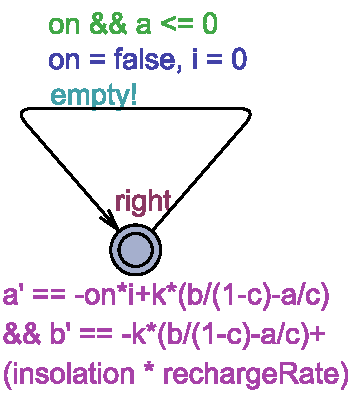
\includegraphics[width=4cm]{graphics/smc_costhandler.pdf} }}%
	\qquad
	\subfloat
	{{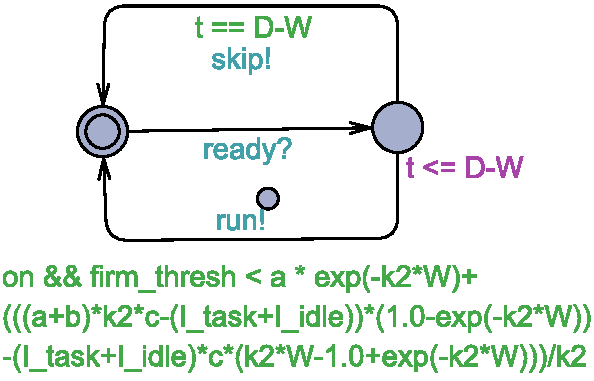
\includegraphics[width=6cm]{graphics/smc_scheduler.pdf} }}%
	\caption{The SMC model's energy source(left) and scheduler(right)}%
	\label{fig:cost_schedule}%
\end{figure}

\begin{figure}[H]%
	\centering
	\subfloat
	{{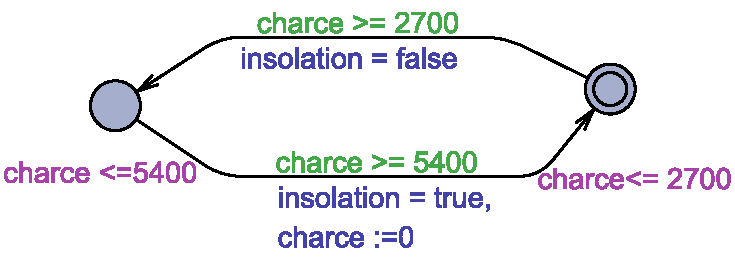
\includegraphics[width=8cm]{graphics/smc_solar.pdf} }}%
	\qquad
	\subfloat
	{{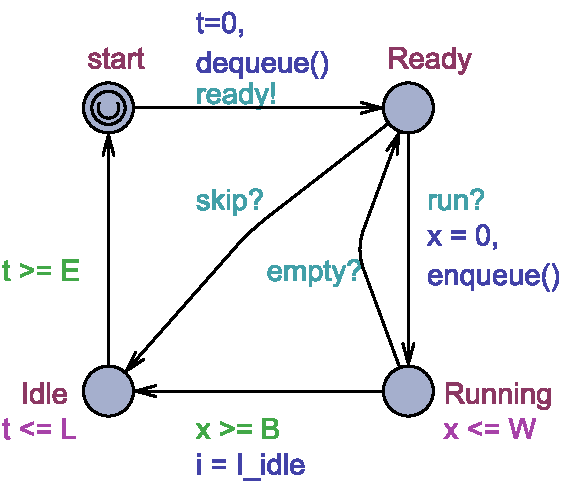
\includegraphics[width=6cm]{graphics/smc_task.pdf} }}%
	\caption{The SMC model's representation of solar panels(left) and a task(right)}%
	\label{fig:solar_task}%
\end{figure}